\chapter{Methodology}
\label{ch:method}

This chapter describes the proposed approach: the system architecture, the formal model of the controller-management problem, the Markov decision process (MDP) solved by the agent, the reward, the Rainbow DQN learner, the GRU forecaster and its integration, and the baselines. Each section ends with the rationale for its main design choices.

\section{System Architecture and Workflow}
\label{sec:architecture}

Figure~\ref{fig:architecture} shows the architecture. It has four parts.
\begin{enumerate}[leftmargin=*]
  \item A \textbf{data layer} turns a Topology Zoo graph into a switch-to-controller delay matrix and supplies a normalised switch-load trace, split chronologically into training, validation and test segments.
  \item A \textbf{controller-management environment}, implemented with the Gymnasium interface~\cite{towers2024gymnasium}, holds the controller states and the switch mapping. It detects overload and underload, exposes the set of currently valid actions, applies the chosen action and returns the next state, a reward and performance metrics.
  \item A \textbf{Rainbow DQN agent}, logically located in the master controller, maps the state to an action.
  \item An optional \textbf{GRU forecaster} predicts near-future switch loads. In \emph{predictive mode} the forecasts are appended to the state and used to anticipate overload.
\end{enumerate}

The same environment code is reused unchanged by the Mininet emulation backend (Section~\ref{sec:mininet-setup}), where it is fed measured instead of trace loads and its decisions are carried out on emulated switches and controller processes.

At each decision interval $t$ the workflow is: (i) observe the state $s_t$; (ii) compute the valid action set $\mathcal{V}(s_t)$; (iii) select $a_t\in\mathcal{V}(s_t)$; (iv) execute $a_t$ and compute the reward $r_t$ from the resulting configuration; (v) advance the traffic trace by one row, recompute controller loads and, in predictive mode, refresh the forecast to produce $s_{t+1}$; and (vi) during training, store the transition and update the network.

\begin{figure}[htbp]
  \centering
  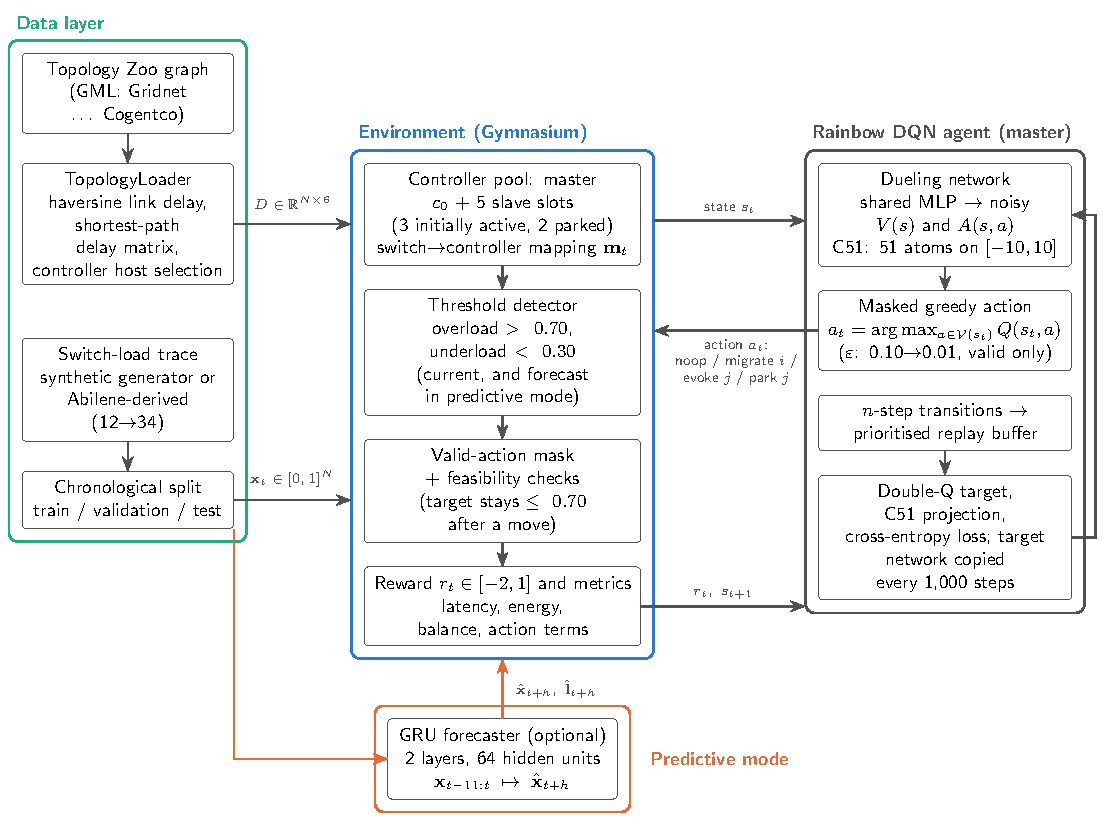
\includegraphics[width=\textwidth]{architecture}
  \caption{Architecture of the proactive controller-management framework. Orange elements are active only in predictive mode.}
  \label{fig:architecture}
\end{figure}

\section{System Model}
\label{sec:system-model}

\paragraph{Topology and controllers.} The network is an undirected graph $G=(\mathcal{S},\mathcal{E})$ with $N=|\mathcal{S}|$ switches. Each link $(u,v)$ has a propagation delay $d_{uv}=\max(\text{dist}_{\text{hav}}(u,v)/200,\ 0.1)$\,ms. Here $\text{dist}_{\text{hav}}$ is the great-circle distance in km between node coordinates, and 200\,km/ms approximates signal speed in fibre; links without coordinates receive 1\,ms. There are $K=6$ controller slots $\mathcal{C}=\{c_0,\dots,c_5\}$ hosted on the six nodes with the highest degree, with ties broken by closeness centrality. Slot $c_0$ is the master controller, which runs the agent and never manages switches. Slots $c_1$--$c_3$ start \emph{active} and $c_4$, $c_5$ start \emph{parked}. Let $D\in\mathbb{R}^{N\times K}$ be the shortest-path delay from each switch to each controller host.

\paragraph{Traffic and controller load.} At interval $t$ the trace supplies $\mathbf{x}_t\in[0,1]^N$, the normalised load of every switch. Let $A_t$ denote the set of active slave controllers and $m_t(i)\in A_t$ the controller of switch $i$. The load of an active controller is the \emph{mean} load of its switches:
\begin{equation}
  \ell_{j,t} = \frac{1}{|\{i:m_t(i)=j\}|}\sum_{i:\,m_t(i)=j} x_{i,t}, \qquad j\in A_t .
  \label{eq:load}
\end{equation}
A mean rather than a sum keeps $\ell_{j,t}$ in $[0,1]$ and comparable with fixed thresholds across topologies whose controllers serve very different numbers of switches. At reset, each switch is assigned to its nearest active controller according to $D$.

\paragraph{Energy model.}
\label{sec:energy}
The energy model follows controller state: the master consumes $E_m=50$\,W, each active slave $E_a=100$\,W and each parked slave $E_p=10$\,W, so $E_t=E_m+|A_t|E_a+|P_t|E_p$, where $P_t$ is the set of parked slaves. The initial configuration consumes 370\,W. This is a relative model used consistently for every policy; it is not a hardware measurement.

\section{Markov Decision Process Formulation}
\label{sec:mdp}

\paragraph{State.} In \emph{current mode} the observation is
\begin{equation}
  s_t = \big[\,\bm{\ell}_t,\ \mathbf{b}_t,\ \mathbf{m}_t\,\big]\in[0,1]^{2K+N},
\end{equation}
where $\bm{\ell}_t\in[0,1]^K$ are the controller loads (zero for parked slots), $\mathbf{b}_t\in\{0,1\}^K$ marks active controllers (the master is always 1), and $\mathbf{m}_t$ holds each switch's controller index divided by $K-1$. In \emph{predictive mode} the GRU forecast $\hat{\mathbf{x}}_{t+h}$ and the forecast controller loads $\hat{\bm{\ell}}_{t+h}$ (Eq.~\ref{eq:load} applied to $\hat{\mathbf{x}}_{t+h}$ under the current mapping) are appended:
\begin{equation}
  s^{\text{pred}}_t = \big[\,\bm{\ell}_t,\ \mathbf{b}_t,\ \mathbf{m}_t,\ \hat{\mathbf{x}}_{t+h},\ \hat{\bm{\ell}}_{t+h}\,\big]\in[0,1]^{2K+2N+K}.
\end{equation}
For OS3E ($N=34$) the state therefore has 46 elements in current mode and 86 in predictive mode.

\paragraph{Actions.} The discrete action space uses \emph{stable slots}, so an action index always means the same thing:
\begin{equation}
  \mathcal{A}=\{0\}\ \cup\ \{1,\dots,N\}\ \cup\ \{N{+}1,\dots,N{+}5\}\ \cup\ \{N{+}6,\dots,N{+}10\},
\end{equation}
namely no-op; migrate switch $i$; evoke slave $c_j$; park slave $c_j$. The size is $|\mathcal{A}|=N+11$, which is 20 actions for Gridnet and 208 for Cogentco. A migrate action names only the switch. The environment chooses the least-loaded feasible active target, which keeps the action space linear in $N$ instead of $N\times K$. Stable slots were introduced after an earlier implementation, in which park/evoke indices depended on the current controller state, was found to give the same index different meanings over time (Appendix~\ref{app:verification}).

\paragraph{Transitions and episodes.} The chosen action changes the mapping and the controller states. The trace then advances by exactly one row, so every step is one decision interval. Episodes last 1,000 steps during training and 500 steps during evaluation, and each episode starts at a specified index of the trace.

\section{Thresholds, Valid Actions and Feasibility}
\label{sec:valid}

An active controller is \emph{overloaded} if $\ell_{j,t}>\theta_{\text{over}}=0.70$ and \emph{underloaded} if $\ell_{j,t}<\theta_{\text{under}}=0.30$. Algorithm~\ref{alg:valid} computes the valid action set. No-op is always valid. Migration and evoking are offered only when some controller is overloaded. Parking is offered only for an underloaded controller whose switches can be absorbed by the remaining active controllers without overloading any of them. A migration is valid only if the chosen target stays at or below $\theta_{\text{over}}$ after the move. When a controller is evoked, the environment immediately moves the most heavily loaded switch of the most overloaded controller onto it, so that the new capacity is used at once.

In predictive mode, the overload set is the union of currently overloaded and \emph{forecast}-overloaded controllers, so migration and evoking can become available before overload occurs. Two conservative rules limit the influence of forecasts: a migration must also keep the target's \emph{forecast} load at or below $\theta_{\text{over}}$, and parking is based on \emph{current} underload only, so a forecast alone never removes capacity.

\begin{algorithm}[htbp]
\caption{Valid-action set $\mathcal{V}(s_t)$}
\label{alg:valid}
\small
\begin{tabbing}
\hspace{1.2em}\=\hspace{1.2em}\=\hspace{1.2em}\=\kill
\textbf{Input:} mapping $m$, active set $A$, parked set $P$, loads $\bm{\ell}$, forecast loads $\hat{\bm{\ell}}$ (predictive mode)\\
1:\> $\mathcal{V}\leftarrow\{0\}$ \hfill \emph{no-op is always valid}\\
2:\> $O\leftarrow\{j\in A:\ell_j>0.70\}$;\quad \textbf{if} predictive \textbf{then} $O\leftarrow O\cup\{j\in A:\hat\ell_j>0.70\}$\\
3:\> $U\leftarrow\{j\in A:\ell_j<0.30\}$ \hfill \emph{current underload only}\\
4:\> \textbf{if} $O\neq\emptyset$ \textbf{then}\\
5:\>\> \textbf{for each} switch $i$ with $m(i)\in O$ \textbf{do}\\
6:\>\>\> $k\leftarrow\arg\min_{j\in A\setminus\{m(i)\}}\ \ell_j$ \quad (predictive: $\max(\ell_j,\hat\ell_j)$)\\
7:\>\>\> \textbf{if} load of $k$ after moving $i$ $\le0.70$ (and forecast load $\le0.70$) \textbf{then} add \emph{migrate}$(i)$\\
8:\>\> add \emph{evoke}$(j)$ for every $j\in P$\\
9:\> \textbf{if} $|A|>1$ \textbf{then}\\
10:\>\> \textbf{for each} $j\in U$ \textbf{do}\\
11:\>\>\> tentatively reassign $j$'s switches, heaviest first, to the least-loaded remaining controller\\
12:\>\>\> \textbf{if} no remaining controller exceeds $0.70$ \textbf{then} add \emph{park}$(j)$\\
13:\> \textbf{return} $\mathcal{V}$
\end{tabbing}
\end{algorithm}

\paragraph{Rationale.} Masking invalid actions~\cite{huang2022masking} keeps the agent from spending experience on impossible actions and keeps it from ever executing an unsafe reassignment. It also means that all policies, learned and baseline, choose from exactly the same legal moves, which keeps the comparison fair. The fixed 0.30/0.70 thresholds were kept unchanged throughout the project so that later implementation fixes were not confounded with changes to the problem definition.

\section{Reward Design}
\label{sec:reward}

The step reward combines three normalised operating costs with action-dependent shaping terms, and is clipped to $[-2,1]$:
\begin{equation}
  r_t=\operatorname{clip}_{[-2,1]}\Big(-\big(0.35\,\tilde L_t+0.35\,\tilde E_t+0.30\,\tilde B_t\big)+\alpha_t-\omega_t\Big),
  \label{eq:reward}
\end{equation}
where
\begin{align}
  \tilde L_t &= \frac{\frac{1}{N}\sum_i D_{i,m_t(i)}}{\max D}, &
  \tilde E_t &= \frac{E_t-E_{\min}}{E_{\max}-E_{\min}}, &
  \tilde B_t &= \frac{\min(\mathrm{CV}(\bm{\ell}_{A_t}),\,2)}{2}.
\end{align}
$\tilde L_t$ is the average switch--controller delay normalised by the largest delay in the topology. $\tilde E_t$ normalises energy between $E_{\min}=190$\,W (one active slave) and $E_{\max}=550$\,W (all five active). $\tilde B_t$ is the coefficient of variation of active-controller loads, capped at 2.

The shaping term $\alpha_t$ (Table~\ref{tab:shaping}) rewards actions that match the conditions observed \emph{before} acting and penalises failed or unjustified ones. A no-op is penalised when overload is present, and also when an underloaded controller exists and more than one controller is active, so that the agent does not learn passivity as a safe default. The anti-oscillation term $\omega_t=1$ applies when a successful park follows a successful evoke (or vice versa) within five steps without an overload to justify it, discouraging rapid flapping of controller state.

\begin{table}[htbp]
\centering
\caption{Action-dependent shaping term $\alpha_t$ (conditions are evaluated on the current state before the action).}
\label{tab:shaping}
\small
\begin{tabular}{@{}lll@{}}
\toprule
\textbf{Action outcome} & \textbf{Condition} & $\bm{\alpha_t}$\\
\midrule
Any non-no-op action fails & -- & $-0.50$\\
Park succeeds & underload present and parking possible & $+0.50$ (else $-0.25$)\\
Evoke succeeds & current overload present & $+0.50$ (else $-0.25$)\\
Migrate succeeds & current overload present & $+0.25$ (else $-0.10$)\\
No-op & current overload present & $-1.00$\\
No-op & underload present and $|A_t|>1$ & $-0.80$ (additive)\\
\bottomrule
\end{tabular}
\end{table}

\paragraph{Rationale.} (i) Normalising every term to $[0,1]$ makes the weights interpretable and keeps per-step rewards within $[-2,1]$, so $n$-step returns stay well inside the fixed C51 support $[-10,10]$. An earlier version with bonuses of about $\pm200$ fell outside that support and was replaced (Appendix~\ref{app:verification}). (ii) Latency and energy receive equal weight because they are the two quantities that parking and migration trade against each other; balance receives slightly less because migration already serves it through the overload terms. (iii) The reward is computed from \emph{actual} current conditions in both modes. A forecast can make an action available early, but cannot make that action look beneficial: a forecast-triggered evoke receives $-0.25$ immediately and must be justified by the lower overload penalties that follow. This prevents the predictive agent from being rewarded merely for trusting its forecaster.

\section{Rainbow DQN Agent}
\label{sec:rainbow}

The agent implements all six Rainbow components~\cite{hessel2018rainbow} in PyTorch~\cite{paszke2019pytorch}.

\paragraph{Network.} A shared feature extractor (two fully connected layers of width $H$ with ReLU) feeds two streams built from noisy linear layers with factorised Gaussian noise ($\sigma_0=0.5$)~\cite{fortunato2018noisy}. The value stream ($H\to H\to51$) and advantage stream ($H\to H\to|\mathcal{A}|\cdot51$) are combined in dueling form~\cite{wang2016dueling},
$z(s,a)=V(s)+A(s,a)-\frac{1}{|\mathcal{A}|}\sum_{a'}A(s,a')$. A softmax over 51 atoms gives a categorical return distribution $p(s,a)$ on the fixed support $\{z_k\}$ spanning $[-10,10]$ (C51~\cite{bellemare2017c51}). The action value is $Q(s,a)=\sum_k z_k\,p_k(s,a)$.

\paragraph{Learning.} Transitions are aggregated into $n$-step returns $R^{(n)}_t=\sum_{k=0}^{n-1}\gamma^k r_{t+k}$ with $\gamma=0.99$, and partial returns are flushed correctly at episode ends. They are stored in a prioritised replay buffer~\cite{schaul2016per} with $\alpha=0.6$ and importance-sampling exponent $\beta$ annealed from 0.4 to 1. For a sampled batch, the online network selects $a^*=\arg\max_a Q_{\text{online}}(s_{t+n},a)$ and the target network evaluates it (double Q-learning~\cite{vanhasselt2016double}). The target distribution of $R^{(n)}_t+\gamma^n z_k$ is projected onto the fixed support, and the loss is the importance-weighted cross-entropy
\begin{equation}
  \mathcal{L}=\mathbb{E}\Big[w_i\Big(-\sum_k \Phi\big(\hat{\mathcal{T}}p_{\text{target}}\big)_k\ \log p_k(s_t,a_t)\Big)\Big].
\end{equation}
The per-sample loss becomes the new priority. Gradients are clipped to norm 10 and optimised with Adam. The target network is copied every 1,000 steps, and gradient updates start after 1,000 warm-up steps, one every four environment steps.

\paragraph{Action selection.} During training, with a small probability $\varepsilon$ decaying exponentially from 0.10 to 0.01 the agent samples uniformly from $\mathcal{V}(s_t)$; otherwise it acts greedily on masked Q-values, $a_t=\arg\max_{a\in\mathcal{V}(s_t)}Q(s_t,a)$, while noisy layers supply state-dependent exploration. During evaluation, noise is disabled (mean weights) and selection is masked greedy, with no learning. Algorithm~\ref{alg:train} summarises training.

\begin{algorithm}[htbp]
\caption{Training the proactive Rainbow DQN agent}
\label{alg:train}
\small
\begin{tabbing}
\hspace{1.2em}\=\hspace{1.2em}\=\hspace{1.2em}\=\kill
\textbf{Input:} training trace $X^{\text{train}}$, topology, mode $\in\{\text{current},\text{predictive}\}$, frozen GRU (predictive), budget $T$, seed\\
1:\> initialise online and target networks, replay buffer $\mathcal{B}$, environment; set all random seeds\\
2:\> $s\leftarrow$ reset(start index $0$)\\
3:\> \textbf{for} $t=0,\dots,T-1$ \textbf{do}\\
4:\>\> $\mathcal{V}\leftarrow$ valid actions (Alg.~\ref{alg:valid});\ \ $a\leftarrow$ random in $\mathcal{V}$ w.p.\ $\varepsilon_t$, else $\arg\max_{a\in\mathcal{V}}Q(s,a)$\\
5:\>\> $(s',r,\text{done})\leftarrow$ env.step$(a)$;\ \ push $(s,a,r,s',\text{done})$ through the $n$-step buffer into $\mathcal{B}$\\
6:\>\> \textbf{if} $t\ge1000$ \textbf{and} $t \bmod 4=0$ \textbf{then} sample prioritised batch; double-Q C51 update; update priorities\\
7:\>\> \textbf{if} $t \bmod 1000=0$ \textbf{then} copy online $\rightarrow$ target\\
8:\>\> $s\leftarrow s'$;\ \ \textbf{if} done \textbf{then} $s\leftarrow$ reset(start index $=1000\cdot\text{episode} \bmod |X^{\text{train}}|$)\\
9:\> save checkpoint and metadata (dimensions, hyperparameters, reward and action-schema versions, seed)
\end{tabbing}
\end{algorithm}

\paragraph{Rationale.} The problem has a large discrete action space (up to 208 actions), sparse and delayed consequences (parking pays off over many steps), and expensive interaction on large topologies. Rainbow addresses these directly: prioritised replay and $n$-step returns propagate rare high-value transitions, double Q-learning and the distributional loss stabilise value estimates, the dueling stream helps when many actions have similar value (most of the time only no-op is reasonable), and noisy layers provide exploration on top of the masked $\varepsilon$-schedule. Policy-gradient methods were not used because a value-based method with masking is a natural fit for a discrete action space of this size, and because it allows a direct methodological comparison with the closest prior work, MOOO-RDQN~\cite{chen2025mooo}. Network width, learning rate, $n$, buffer and batch size scale with topology size (Table~\ref{tab:hyper}).

\section{GRU Traffic Forecaster}
\label{sec:gru}

\paragraph{Model.} The forecaster maps the last $H_{\text{hist}}=12$ switch-load vectors to the load vector $h$ steps ahead: $\hat{\mathbf{x}}_{t+h}=f_\phi(\mathbf{x}_{t-11},\dots,\mathbf{x}_t)$. It is a two-layer GRU~\cite{cho2014gru} with hidden size 64 and dropout 0.1, whose last hidden state passes through a $64\to64\to N$ MLP. Inputs and targets are standardised per switch with statistics computed \emph{only} from the training split. Training minimises MSE with Adam (learning rate $10^{-3}$, batch 128, gradient clip 5) for up to 50 epochs, with early stopping (patience 8) on validation loss; the best validation checkpoint is kept. Every forecaster is compared with a \emph{persistence} baseline, $\hat{\mathbf{x}}_{t+h}=\mathbf{x}_t$, on the same validation windows, using MAE, RMSE and precision/recall/F1 for predicting a switch load above 0.70.

\paragraph{Integration.} The trained GRU is frozen and wrapped as a predictor. The environment keeps a rolling 12-step history, primed from the preceding rows of the trace at each reset, and calls the predictor after every trace update. Predictions are clipped to $[0,1]$ and converted to forecast controller loads under the current mapping. Forecasts influence the agent in exactly two ways: they extend the state, and they enlarge the overload set used for migration and evoking (Section~\ref{sec:valid}). The forecaster is not the decision-maker, and its errors are not rewarded or penalised directly.

\paragraph{Rationale.} A GRU has fewer parameters than an LSTM~\cite{hochreiter1997lstm} with similar sequence-modelling ability~\cite{chung2014gru}, which suits a forecaster that must run once per decision step. Freezing it keeps the forecasting and control problems separable. This allows the forecaster to be judged against persistence on its own and makes the current-versus-predictive comparison an ablation of the forecast input alone.

\section{Baseline Policies}
\label{sec:baselines}

Three untrained baselines use the same environment, action API and valid-action mask:
\begin{itemize}[leftmargin=*]
  \item \textbf{Threshold.} If a controller is currently overloaded, evoke the lowest-index parked controller; if none is parked, migrate a valid switch from the most loaded overloaded controller. Otherwise, if an underloaded controller can be parked, park the least-loaded one. Otherwise do nothing. This encodes the usual reactive rule-based practice.
  \item \textbf{Random-valid.} Sample uniformly from $\mathcal{V}(s_t)$. It isolates the value of \emph{choosing} among legal actions from the value of the action set itself.
  \item \textbf{No-op.} Never act; the nearest-controller assignment and the initial three active controllers persist. It is the static-placement reference.
\end{itemize}
In predictive mode the baselines run in the predictive environment. The threshold rule still triggers on \emph{current} overload, but its candidate migrations must pass the stricter predictive feasibility check, and random-valid samples from a valid set that forecasts can enlarge. Baseline trajectories therefore differ between modes even though their rules are unchanged. Learned policies are therefore always compared with baselines \emph{in the same observation mode}.
